\documentclass{beamer}
\usetheme[numbering=progressbar]{focus}
\usepackage{tikz}
\usetikzlibrary{positioning}
\usetikzlibrary{shapes,arrows}
\usepackage{transparent}
\usepackage{fancyvrb}
\usepackage{listings}
\definecolor{main}{RGB}{47, 161, 219}
%\definecolor{textcolor}{RGB}{128, 128, 128}
\definecolor{background}{RGB}{240, 247, 255}
\definecolor{textcolor}{RGB}{85, 87, 83}
\title{Passive SSH, a Fast-Lookup Database of SSH Key Materials to Support Incident Response}
\subtitle{}
\author{Alexandre Dulaunoy - Aurelien Thirion}
\titlegraphic{
\includegraphics[scale=0.6]{passivessh.pdf}}
\institute{Team CIRCL \\ \url{https://www.d4-project.org/}}
\date{2020-11-16}

\begin{document}
    \begin{frame}
        \maketitle
    \end{frame}

\begin{frame}
        \frametitle{Problem statement}
        \begin{itemize}
                \item CIRCL (and other CSIRTs) have their own passive DNS\footnote{\url{https://www.circl.lu/services/passive-dns/}} and passive SSL{\footnote{\url{https://www.circl.lu/services/passive-ssl/}}} database
                \item Historical data is a companion to incident response, infrastructure attribution and threat intelligence at large
                \item {\bf SSH is a major protocol for remote management} (for normal users but also attackers)
                \item SSH protocol provides a significant {\bf number of fingerprints} to track similar infrastructures (e.g. from banners to key fingerprints)
        \end{itemize}
\end{frame}

\begin{frame}
        \frametitle{Passive SSH design}
        \begin{itemize}
                \item A fast-lookup database to find SSH key per IP, fingerprint or hassh\footnote{\url{https://github.com/salesforce/hassh}}
                \item Supporting the storage of the key materials, key types and banners
                \item {\bf Lightweight design} and supporting different kind of importers (scanner, network capture)
                \item The system can be used externally (for Internet-wide scan) or internally (for internal network ssh infrastructure scanning)
                \item Supporting IPv4, IPv6 but also Tor onion addresses or random TCP ports
        \end{itemize}
\end{frame}

\begin{frame}
        \frametitle{Passive SSH open source software}
        \begin{itemize}
                \item Software written in Python 3 and released as an open source project\footnote{\url{https://github.com/D4-project/passive-ssh}}
                \item The database is a {\bf Redis-compatible backend} (you can use Redis, kv-rocks or any compatible Redis backend)
                \item A sample SSH scanner is included to scan small networks or internal infrastructure
                \item CIRCL provides a {\bf database from an Internet-wide scan} (access can be requested for FIRST, TF-CSIRT and CNW members)
        \end{itemize}
\end{frame}

\begin{frame}
        \frametitle{What do you store? or What can I lookup?}
        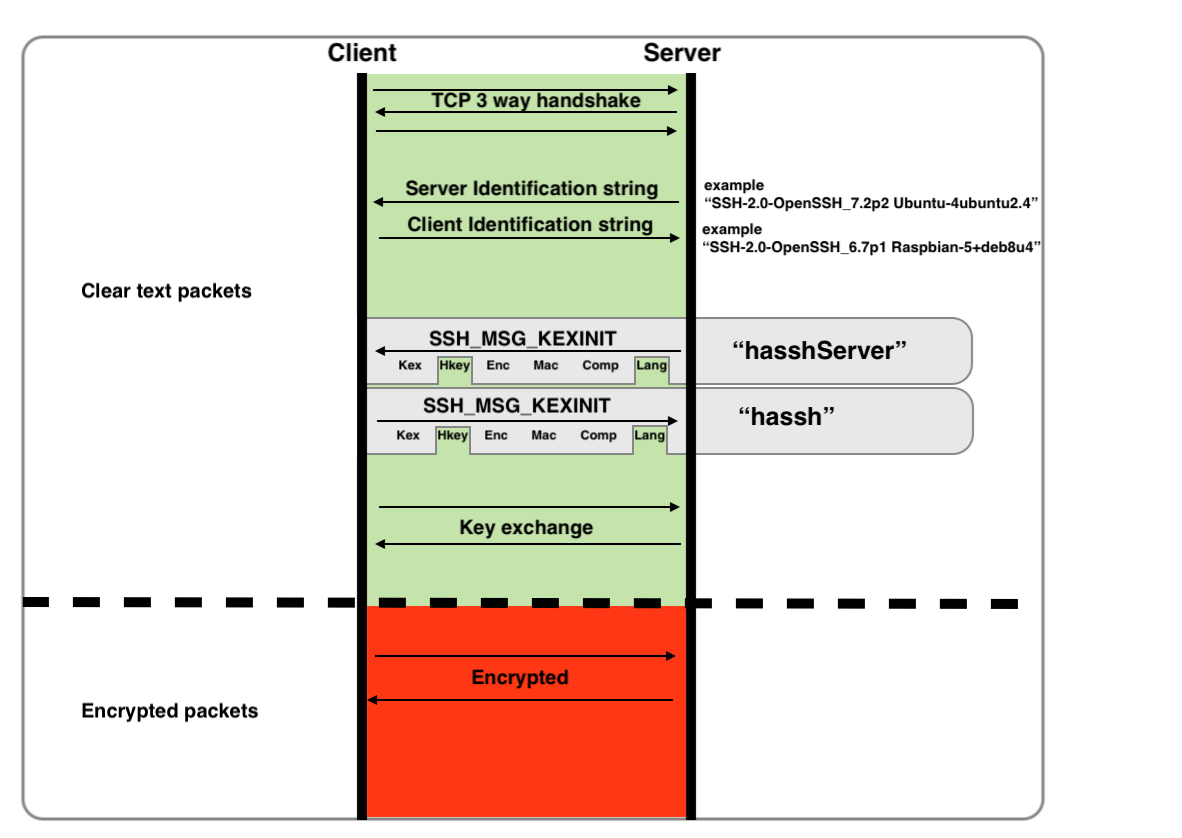
\includegraphics[scale=0.3]{sshhandshake.png}
\end{frame}

\begin{frame}[t,fragile]
        \frametitle{}
\lstdefinelanguage{JavaScript}{
  keywords={typeof, new, true, false, catch, function, return, null, catch, switch, var, if, in, while, do, else, case, break},
  keywordstyle=\color{blue}\bfseries,
  ndkeywords={class, export, boolean, throw, implements, import, this},
  ndkeywordstyle=\color{darkgray}\bfseries,
  identifierstyle=\color{black},
  sensitive=false,
  comment=[l]{//},
  morecomment=[s]{/*}{*/},
  commentstyle=\color{purple}\ttfamily,
  stringstyle=\color{red}\ttfamily,
  morestring=[b]',
  morestring=[b]"
}
\lstset{
   language=JavaScript,
   backgroundcolor=\color{lightgray},
   extendedchars=true,
   basicstyle=\footnotesize\ttfamily,
   showstringspaces=false,
   showspaces=false,
   numbers=left,
   numberstyle=\footnotesize,
   numbersep=9pt,
   tabsize=2,
   breaklines=true,
   showtabs=false,
   captionpos=b
}
\lstset{breaklines=true, language=JavaScript}
\begin{lstlisting}
curl -s http://127.0.0.1:8500/banners | jq .
{
  "banners": {
    "SSH-2.0-OpenSSH_7.6p1 Ubuntu-4ubuntu0.3": 14522,
    "SSH-2.0-OpenSSH_7.4": 8036,
    "SSH-2.0-OpenSSH_7.9p1 Debian-10+deb10u2": 4563,
    "SSH-2.0-OpenSSH_7.2p2 Ubuntu-4ubuntu2.8": 4464,
    "SSH-2.0-OpenSSH_7.4p1 Debian-10+deb9u7": 4301,
    "SSH-2.0-OpenSSH_5.3": 2930,
    "SSH-2.0-OpenSSH_8.2p1 Ubuntu-4ubuntu0.1": 2901,
    "SSH-2.0-OpenSSH_7.2p2 Ubuntu-4ubuntu2.10": 2669,
    "SSH-2.0-OpenSSH_6.7p1 Debian-5+deb8u8": 2295,
    "SSH-2.0-OpenSSH_7.4p1 Debian-10+deb9u6": 1192,
    "SSH-2.0-OpenSSH_6.6.1p1 Ubuntu-2ubuntu2.13": 1107,
    "SSH-2.0-OpenSSH_6.7p1 Debian-5+deb8u3": 1024,
\end{lstlisting}

\end{frame}


\begin{frame}[t,fragile]
        \frametitle{}
\lstdefinelanguage{JavaScript}{
  keywords={typeof, new, true, false, catch, function, return, null, catch, switch, var, if, in, while, do, else, case, break},
  keywordstyle=\color{blue}\bfseries,
  ndkeywords={class, export, boolean, throw, implements, import, this},
  ndkeywordstyle=\color{darkgray}\bfseries,
  identifierstyle=\color{black},
  sensitive=false,
  comment=[l]{//},
  morecomment=[s]{/*}{*/},
  commentstyle=\color{purple}\ttfamily,
  stringstyle=\color{red}\ttfamily,
  morestring=[b]',
  morestring=[b]"
}
\lstset{
   language=JavaScript,
   backgroundcolor=\color{lightgray},
   extendedchars=true,
   basicstyle=\footnotesize\ttfamily,
   showstringspaces=false,
   showspaces=false,
   numbers=left,
   numberstyle=\footnotesize,
   numbersep=9pt,
   tabsize=2,
   breaklines=true,
   showtabs=false,
   captionpos=b
}
\lstset{breaklines=true, language=JavaScript}
\begin{lstlisting}
curl -s "http://127.0.0.1:8500/banner/hosts/SSH-2.0-OpenSSH_6.7p1%20OVH-rescue"  | jq .
{
  "banner": "SSH-2.0-OpenSSH_6.7p1 OVH-rescue",
  "hosts": [
    "188.165.216.153",
    "137.74.204.16",
    "188.165.233.197",
    "188.165.199.211",
    "188.165.192.121",
    "137.74.204.58",
    "188.165.224.149",
    "188.165.211.205",
    "188.165.216.162",
    "188.165.216.155",
    "188.165.194.193",
\end{lstlisting}

\end{frame}

\begin{frame}[t,fragile]
        \frametitle{}
\lstdefinelanguage{JavaScript}{
  keywords={typeof, new, true, false, catch, function, return, null, catch, switch, var, if, in, while, do, else, case, break},
  keywordstyle=\color{blue}\bfseries,
  ndkeywords={class, export, boolean, throw, implements, import, this},
  ndkeywordstyle=\color{darkgray}\bfseries,
  identifierstyle=\color{black},
  sensitive=false,
  comment=[l]{//},
  morecomment=[s]{/*}{*/},
  commentstyle=\color{purple}\ttfamily,
  stringstyle=\color{red}\ttfamily,
  morestring=[b]',
  morestring=[b]"
}
\lstset{
   language=JavaScript,
   backgroundcolor=\color{lightgray},
   extendedchars=true,
   basicstyle=\footnotesize\ttfamily,
   showstringspaces=false,
   showspaces=false,
   numbers=left,
   numberstyle=\footnotesize,
   numbersep=9pt,
   tabsize=2,
   breaklines=true,
   showtabs=false,
   captionpos=b
}
\lstset{breaklines=true, language=JavaScript}
\begin{lstlisting}
curl -s "http://127.0.0.1:8500/banner/hosts/SSH-2.0-lancom"  | jq .
{
  "banner": "SSH-2.0-lancom",
  "hosts": [
    "89.1.181.237",
    "89.0.231.177",
    "91.0.158.6",
    "91.0.54.88",
    "91.0.146.13",
    "91.1.54.42",
    "91.1.23.189",
    "89.1.29.178",
    "91.0.184.142",
    "89.1.183.80",
    "89.1.142.156",
    "89.1.31.148",

\end{lstlisting}
\end{frame}


\begin{frame}[t,fragile]
        \frametitle{}
\lstdefinelanguage{JavaScript}{
  keywords={typeof, new, true, false, catch, function, return, null, catch, switch, var, if, in, while, do, else, case, break},
  keywordstyle=\color{blue}\bfseries,
  ndkeywords={class, export, boolean, throw, implements, import, this},
  ndkeywordstyle=\color{darkgray}\bfseries,
  identifierstyle=\color{black},
  sensitive=false,
  comment=[l]{//},
  morecomment=[s]{/*}{*/},
  commentstyle=\color{purple}\ttfamily,
  stringstyle=\color{red}\ttfamily,
  morestring=[b]',
  morestring=[b]"
}
\lstset{
   language=JavaScript,
   backgroundcolor=\color{lightgray},
   extendedchars=true,
   basicstyle=\tiny\ttfamily,
   showstringspaces=false,
   showspaces=false,
   numbers=left,
   numberstyle=\footnotesize,
   numbersep=9pt,
   tabsize=2,
   breaklines=true,
   showtabs=false,
   captionpos=b
}
\lstset{breaklines=true, language=JavaScript}
\begin{lstlisting}
 curl -s "http://127.0.0.1:8500/host/ssh/89.1.181.237"  | jq .
{
  "first_seen": "20201116",
  "last_seen": "20201116",
  "port": 22,
  "banner": [
    "SSH-2.0-lancom"
  ],
  "hassh": {
    "deabc869d8b35c2fbef0831b838bf196": [
      "{\"key\": [\"rsa-sha2-512\", \"rsa-sha2-256\", \"ssh-rsa\", \"ssh-dss\"], \"encrypt\": [\"aes256-ctr\", \"aes192-ctr\", \"aes128-ctr\", \"aes256-cbc\", \"aes192-cbc\", \"aes128-cbc\", \"blowfish-ctr\", \"
blowfish-cbc\", \"arcfour256\", \"arcfour128\", \"arcfour\", \"3des-ctr\", \"3des-cbc\"], \"mac\": [\"hmac-sha2-512\", \"hmac-sha2-512-96\", \"hmac-sha2-256\", \"hmac-sha2-256-96\", \"hmac-sha1\", \"hmac-sha1-96
\", \"hmac-md5\", \"hmac-md5-96\"], \"compress\": [\"none\", \"zlib\"], \"lang\": []}"
    ]
  },
  "keys": [
    {
      "type": "ssh-rsa",
      "fingerprint": "af:80:1e:6f:5a:cf:f3:6e:7d:2a:aa:a5:f3:05:0e:1b"
    },
    {
      "type": "ssh-dss",
      "fingerprint": "8a:b9:c0:a6:b3:20:de:86:f6:10:97:8e:27:be:f1:ea"
    }
  ]
}
\end{lstlisting}
\end{frame}

\begin{frame}[t,fragile]
        \frametitle{}
\lstdefinelanguage{JavaScript}{
  keywords={typeof, new, true, false, catch, function, return, null, catch, switch, var, if, in, while, do, else, case, break},
  keywordstyle=\color{blue}\bfseries,
  ndkeywords={class, export, boolean, throw, implements, import, this},
  ndkeywordstyle=\color{darkgray}\bfseries,
  identifierstyle=\color{black},
  sensitive=false,
  comment=[l]{//},
  morecomment=[s]{/*}{*/},
  commentstyle=\color{purple}\ttfamily,
  stringstyle=\color{red}\ttfamily,
  morestring=[b]',
  morestring=[b]"
}
\lstset{
   language=JavaScript,
   backgroundcolor=\color{lightgray},
   extendedchars=true,
   basicstyle=\footnotesize\ttfamily,
   showstringspaces=false,
   showspaces=false,
   numbers=left,
   numberstyle=\footnotesize,
   numbersep=9pt,
   tabsize=2,
   breaklines=true,
   showtabs=false,
   captionpos=b
}
\lstset{breaklines=true, language=JavaScript}
\begin{lstlisting}
curl -s "http://127.0.0.1:8500/fingerprint/all/af:80:1e:6f:5a:cf:f3:6e:7d:2a:aa:a5:f3:05:0e:1b"  | jq .
{
  "type": "ssh-rsa",
  "first_seen": "20201116",
  "last_seen": "20201116",
  "base64": "ssh-rsa AAAAB3NzaC1yc2EAAAABEQAAAQEAwe/8ooNGMyQCYTYcDlAAj1Da3e4uPbLNBA7zs/oKdeS9JhuJBO5oN0rwKk9B7Y429AL3OHHZUPVQMJ2Rt+fEfObYtLt+BI+289/DYdddUNxX3gU80rF4qiz1uQJ1FjcyW+LN1y219DE9rSshjY6aNPUshDhRuGnBxS
NMJCl3pM6uxPnUhirccpobnHzO9C2cFAIMRGuy1/iJM/fwngGAlxYqtPJ8Pff7rTTcDrPF7YB7STSQXvBTgiwCHVEuxyQaX7Aik5BM0A0DHDrwf6VHDbqWXK6AAM+01W8j1b+lN+yzT4+EZbQJ4kQKfNb8aGWAcHacjs9VOfr4w79ynz/lPQ==",
  "fingerprint": "af:80:1e:6f:5a:cf:f3:6e:7d:2a:aa:a5:f3:05:0e:1b",
  "hosts": [
    "89.1.181.237"
  ]
}
\end{lstlisting}
\end{frame}


\begin{frame}
        \frametitle{Monitoring Attacker Infrastructure}
        \begin{itemize}
                \item {\bf Attackers are also system administrators} and use SSH to manage their infrastructure
                \item Some SSH installation are used as back-door on different ports
                \item {\bf Understanding attacker infrastructure}\footnote{A nice complement to Chapter 4 : Attack Infrastructure in Attribution of Advanced Persistent Threats, Timo Steffens} by looking at SSH banners, keys and fingerprints
                \item SSH cryptographic keys are renewed less often than TLS certificates
        \end{itemize}
\end{frame}

\begin{frame}
        \frametitle{Uncloaking Tor hidden services with Passive SSH}
        \begin{itemize}
                \item We collected a set of Tor onion addresses (~60K) using the AIL framework
                \item Then we scanned for SSH on those onion addresses
                \item Finding {\bf common set of fingerprints} between onion addresses and Internet-wide scan in Passive SSH
        \end{itemize}
\end{frame}

\begin{frame}
        \frametitle{What's next?}
        \begin{itemize}
               \item A MISP module to get Passive {\bf SSH expansion and pivots in MISP project}
               \item Add SSH correlation in AIL framework for crawled Tor hidden services\footnote{\url{https://github.com/ail-project/ail-framework}}
               \item Pcap feeder to Passive SSH
               \item Review of cryptographic materials\footnote{\url{https://github.com/D4-project/snake-oil-crypto}} from existing Passive SSH database
               \item Improvement of the Passive SSH code base and release of version 1.0
        \end{itemize}
\end{frame}

\begin{frame}
\frametitle{Contact}
\begin{itemize}
        \item Get in touch if you want to get access to the {\bf Passive SSH database} (you need to be a FIRST.org, TF-CSIRT or CNW member)
\item Contact: info@circl.lu
\item Source code: \url{https://github.com/D4-project/passive-ssh} -  \url{https://twitter.com/d4_project}
\end{itemize}
\end{frame}


\end{document}
